\section{Введение}

В данной лабораторной работе рассматриваются методы анализа устойчивости нелинейных динамических систем с использованием функций Ляпунова, а также синтез стабилизирующих регуляторов на основе линейных матричных неравенств (LMI).

Основные задачи работы:
\begin{enumerate}
\item Анализ устойчивости пяти различных нелинейных систем с использованием квадратичных функций Ляпунова
\item Исследование условий асимптотической устойчивости скалярной системы специального вида
\item Синтез линейного регулятора через LMI для обеспечения экспоненциальной устойчивости
\item Определение ограничивающих условий на параметры системы для обеспечения устойчивости
\item Анализ системы с линейным управлением по состоянию
\end{enumerate}

Работа демонстрирует применение теоретических методов анализа устойчивости к практическим задачам управления нелинейными системами.

\section{Задача 1. Анализ устойчивости с квадратичными функциями Ляпунова}

Для каждой из следующих систем используем кандидат квадратичной функции Ляпунова $V(x) = x_1^2 + x_2^2$ (для скалярной системы $V(x) = x^2$), чтобы показать, что начало координат асимптотически устойчиво, и определить, в каких случаях система глобально устойчива.

\subsection{Система 1}

Рассмотрим систему:
\begin{align}
\dot{x}_1 &= -x_1 + x_1 x_2 \\
\dot{x}_2 &= -2x_2
\end{align}

Выберем функцию Ляпунова $V(x) = x_1^2 + x_2^2$. Вычислим производную по времени:
\begin{align}
\dot{V} &= 2x_1 \dot{x}_1 + 2x_2 \dot{x}_2 \\
&= 2x_1(-x_1 + x_1 x_2) + 2x_2(-2x_2) \\
&= -2x_1^2 + 2x_1^2 x_2 - 4x_2^2 \\
&= -2(x_1^2 + x_2^2) + 2x_1^2 x_2
\end{align}

\textbf{Анализ устойчивости:}
\begin{itemize}
\item В малой окрестности начала координат член $2x_1^2 x_2$ мал по сравнению с $-2(x_1^2 + x_2^2)$
\item Поэтому $\dot{V} < 0$ локально в окрестности начала координат
\item Система \textbf{локально асимптотически устойчива}
\item При больших значениях $|x_2|$ член $2x_1^2 x_2$ может доминировать, поэтому система \textbf{НЕ глобально устойчива}
\end{itemize}

\subsection{Система 2}

Рассмотрим систему:
\begin{align}
\dot{x}_1 &= -x_2 - x_1(1 - x_1^2 - x_2^2) \\
\dot{x}_2 &= x_1 - x_2(1 - x_1^2 - x_2^2)
\end{align}

С функцией Ляпунова $V(x) = x_1^2 + x_2^2$:
\begin{align}
\dot{V} &= 2x_1 \dot{x}_1 + 2x_2 \dot{x}_2 \\
&= 2x_1[-x_2 - x_1(1 - x_1^2 - x_2^2)] + 2x_2[x_1 - x_2(1 - x_1^2 - x_2^2)] \\
&= -2x_1 x_2 - 2x_1^2(1 - x_1^2 - x_2^2) + 2x_1 x_2 - 2x_2^2(1 - x_1^2 - x_2^2) \\
&= -2(x_1^2 + x_2^2)(1 - x_1^2 - x_2^2)
\end{align}

\textbf{Анализ устойчивости:}
\begin{itemize}
\item Внутри единичного круга ($x_1^2 + x_2^2 < 1$): $\dot{V} < 0$
\item На единичном круге ($x_1^2 + x_2^2 = 1$): $\dot{V} = 0$
\item Вне единичного круга ($x_1^2 + x_2^2 > 1$): $\dot{V} > 0$
\item Система \textbf{локально асимптотически устойчива}
\item Область притяжения ограничена единичным кругом, поэтому система \textbf{НЕ глобально устойчива}
\end{itemize}

\subsection{Система 3}

Рассмотрим систему:
\begin{align}
\dot{x}_1 &= x_2(1 - x_1^2) - 2x_1 \\
\dot{x}_2 &= -(x_1 + x_2)(1 - x_1^2)
\end{align}

С функцией Ляпунова $V(x) = x_1^2 + x_2^2$:
\begin{align}
\dot{V} &= 2x_1[x_2(1 - x_1^2) - 2x_1] + 2x_2[-(x_1 + x_2)(1 - x_1^2)] \\
&= 2x_1 x_2(1 - x_1^2) - 4x_1^2 - 2x_1 x_2(1 - x_1^2) - 2x_2^2(1 - x_1^2) \\
&= -4x_1^2 - 2x_2^2(1 - x_1^2)
\end{align}

\textbf{Анализ устойчивости:}
\begin{itemize}
\item В малой окрестности начала координат ($|x_1| < 1$): $\dot{V} < 0$
\item Система \textbf{локально асимптотически устойчива}
\item При больших значениях $|x_1|$ знак $\dot{V}$ может измениться, поэтому система \textbf{НЕ глобально устойчива}
\end{itemize}

\subsection{Система 4}

Рассмотрим систему:
\begin{align}
\dot{x}_1 &= -3x_1 - x_2 \\
\dot{x}_2 &= 2x_1 - x_2^3
\end{align}

С функцией Ляпунова $V(x) = x_1^2 + x_2^2$:
\begin{align}
\dot{V} &= 2x_1(-3x_1 - x_2) + 2x_2(2x_1 - x_2^3) \\
&= -6x_1^2 - 2x_1 x_2 + 4x_1 x_2 - 2x_2^4 \\
&= -6x_1^2 + 2x_1 x_2 - 2x_2^4
\end{align}

\textbf{Анализ устойчивости:}
\begin{itemize}
\item $\dot{V} = -6x_1^2 + 2x_1 x_2 - 2x_2^4$
\item Для анализа знака рассмотрим квадратичную форму по $x_1$: $-6x_1^2 + 2x_1 x_2$
\item Дискриминант: $D = (2x_2)^2 - 4(-6)(0) = 4x_2^2 \geq 0$
\item Максимальное значение: $\frac{4x_2^2}{4 \cdot 6} = \frac{x_2^2}{6}$
\item Поэтому $-6x_1^2 + 2x_1 x_2 \leq \frac{x_2^2}{6}$
\item $\dot{V} \leq \frac{x_2^2}{6} - 2x_2^4 = x_2^2(\frac{1}{6} - 2x_2^2)$
\item При $|x_2| < \frac{1}{\sqrt{12}}$: $\dot{V} < 0$
\item При $|x_2| \geq \frac{1}{\sqrt{12}}$: $\dot{V} \leq -\frac{11}{6}x_2^2 < 0$
\item Система \textbf{глобально асимптотически устойчива}
\end{itemize}

\subsection{Система 5}

Рассмотрим скалярную систему:
\begin{equation}
\dot{x} = -\arctan(x)
\end{equation}

С функцией Ляпунова $V(x) = x^2$:
\begin{align}
\dot{V} &= 2x \dot{x} = 2x(-\arctan(x)) = -2x\arctan(x)
\end{align}

\textbf{Анализ устойчивости:}
\begin{itemize}
\item Для $x > 0$: $\arctan(x) > 0$, поэтому $\dot{V} < 0$
\item Для $x < 0$: $\arctan(x) < 0$, поэтому $\dot{V} < 0$
\item При $x = 0$: $\dot{V} = 0$
\item Система \textbf{глобально асимптотически устойчива}
\end{itemize}

\subsection{Результаты анализа}

\begin{figure}[H]
\centering
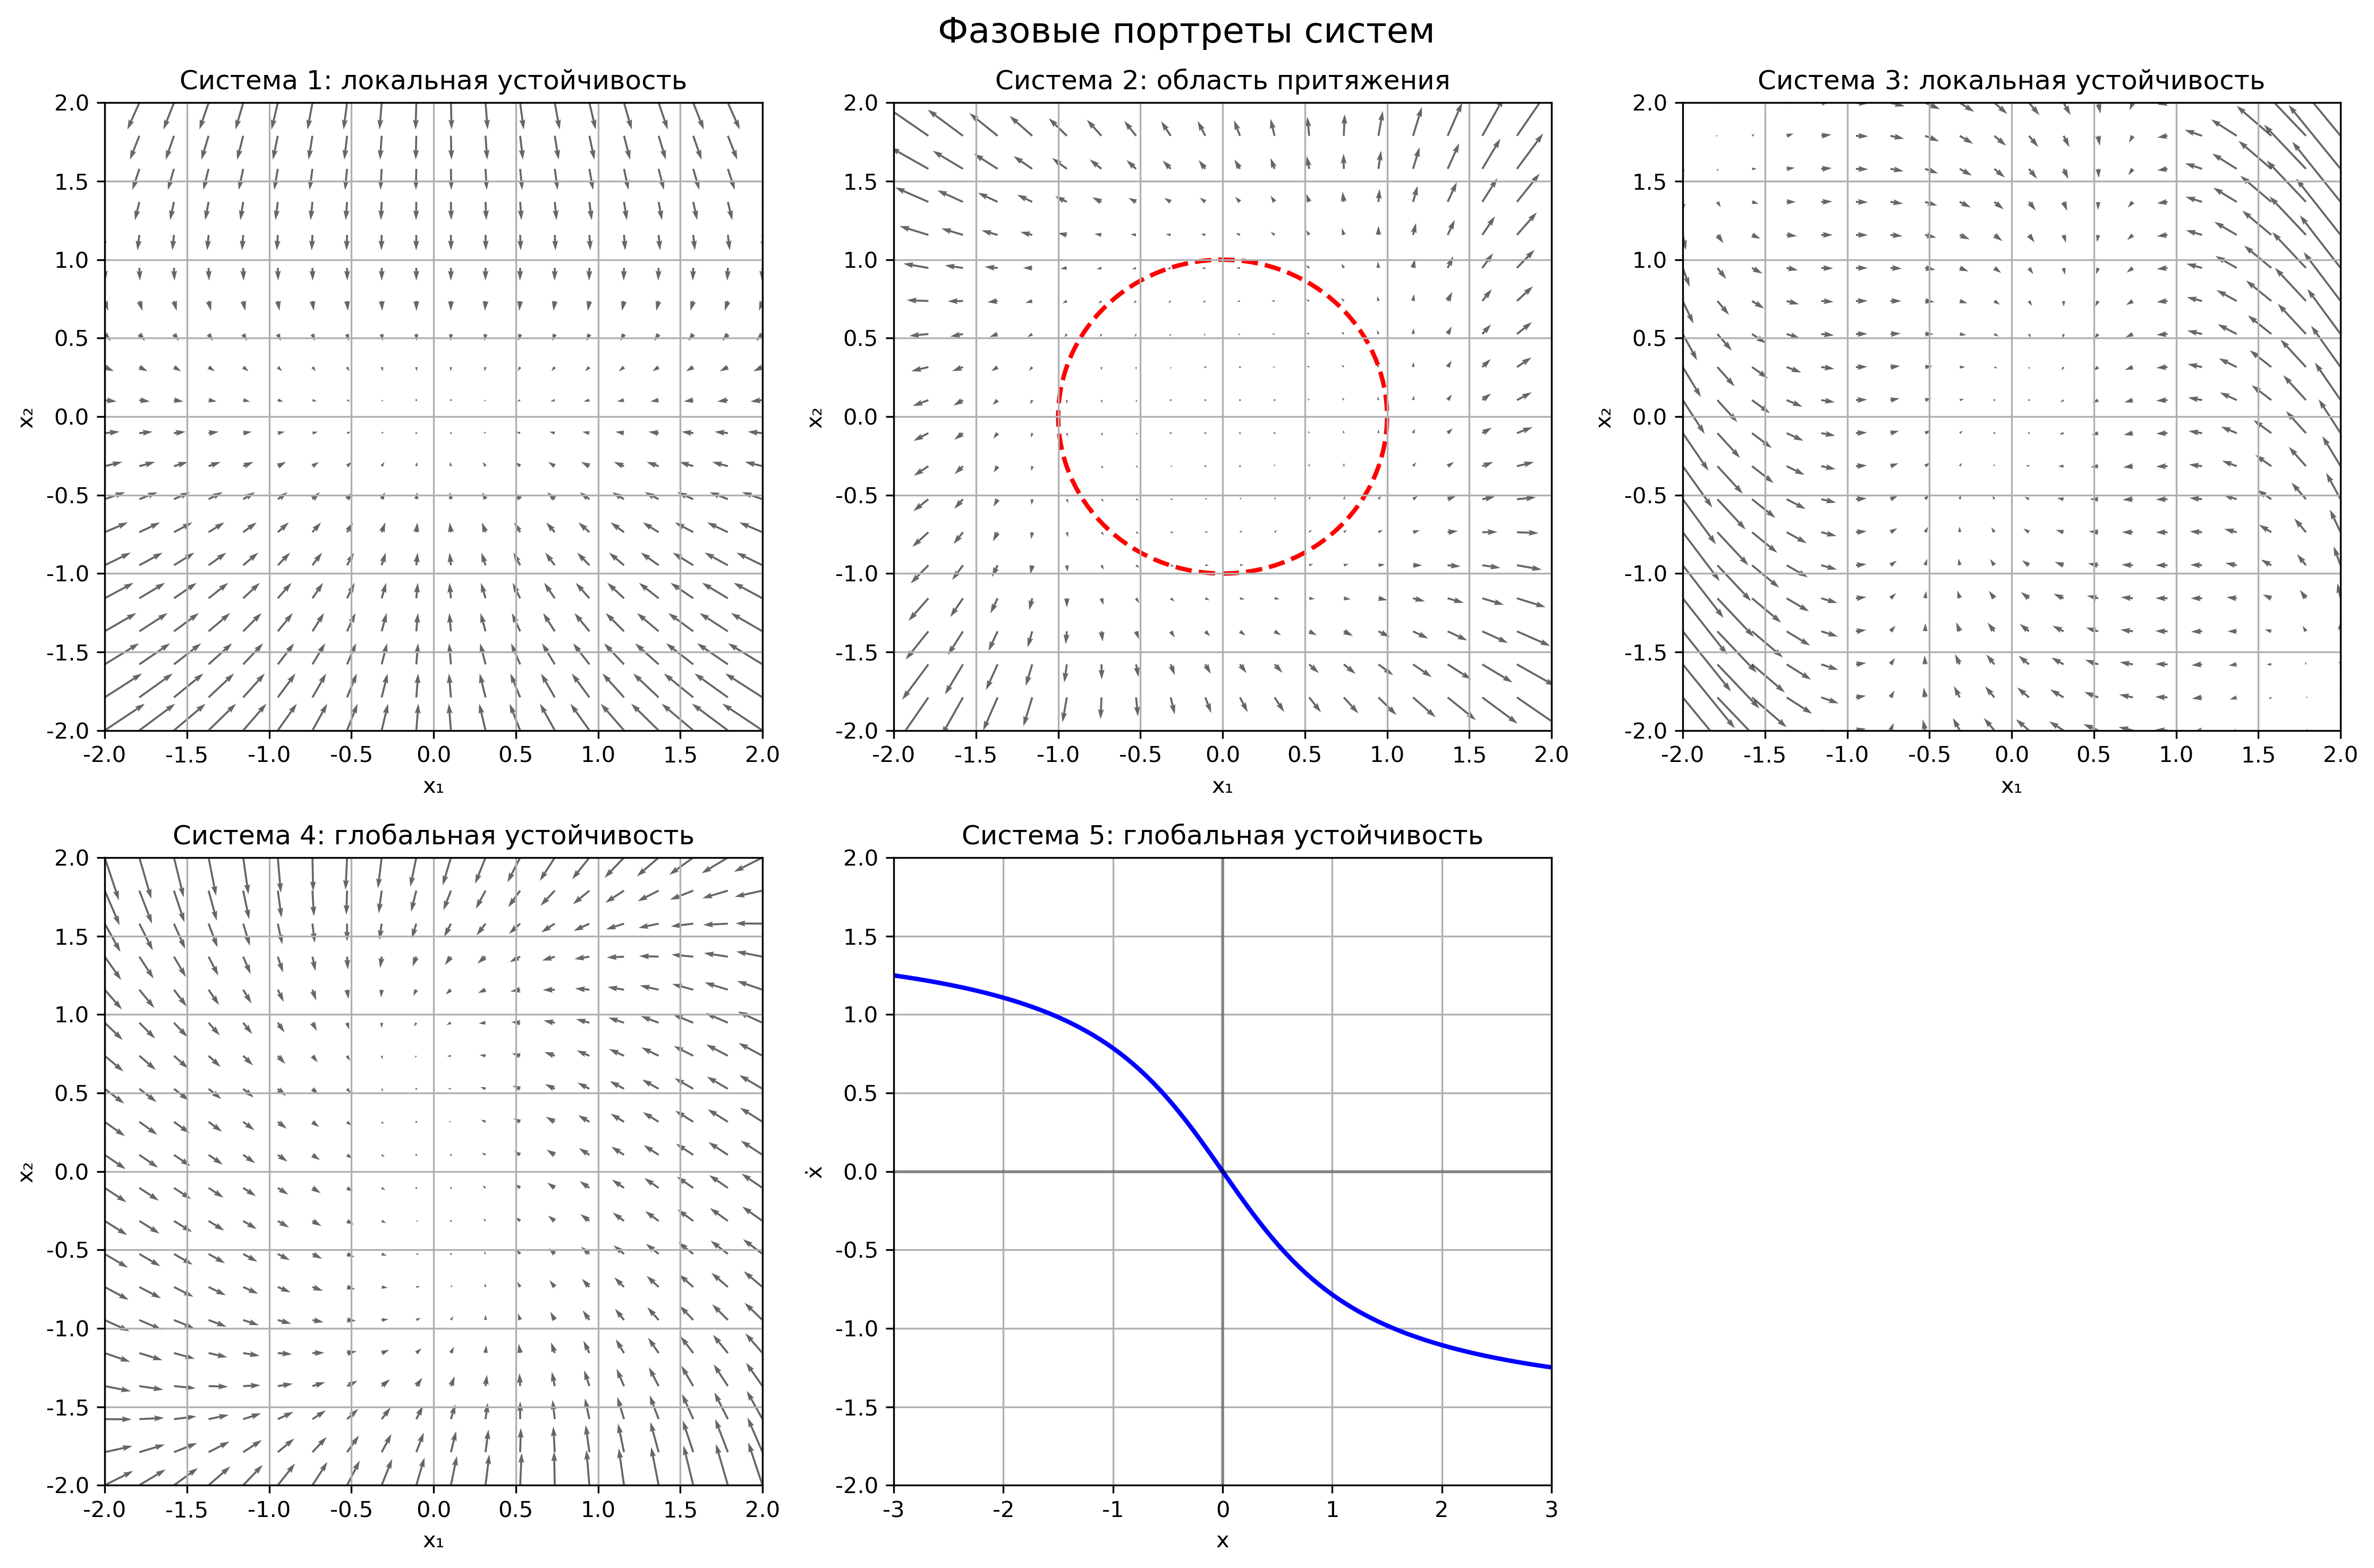
\includegraphics[width=0.9\textwidth]{task1/phase_portraits.png}
\caption{Фазовые портреты систем для анализа устойчивости}
\label{fig:phase_portraits}
\end{figure}

\textbf{Сводка результатов:}
\begin{itemize}
\item \textbf{Система 1}: локально асимптотически устойчива
\item \textbf{Система 2}: локально асимптотически устойчива (область притяжения - единичный круг)
\item \textbf{Система 3}: локально асимптотически устойчива
\item \textbf{Система 4}: глобально асимптотически устойчива
\item \textbf{Система 5}: глобально асимптотически устойчива
\end{itemize}

\textbf{Глобально устойчивые системы:} только системы 4 и 5.

\section{Задача 2. Условия асимптотической устойчивости скалярной системы}

Рассмотрим скалярную систему:
\begin{equation}
\dot{x} = ax^p + h(x)
\end{equation}
где $p$ — натуральное число, а $h(x)$ удовлетворяет условию $|h(x)| \leq k|x|^{p+1}$ в некоторой окрестности точки начала координат.

Требуется определить условия, при которых система асимптотически устойчива.

\subsection{Анализ устойчивости}

Рассмотрим различные случаи в зависимости от значения параметра $a$ и четности $p$.

\subsubsection{Случай 1: $p$ — четное число}

При четном $p$ имеем $x^p \geq 0$ для всех $x$.

\textbf{Если $a < 0$:}
\begin{itemize}
\item $ax^p \leq 0$ для всех $x$
\item В малой окрестности начала координат: $|h(x)| \leq k|x|^{p+1} \ll |ax^p|$
\item Поэтому $\dot{x} \approx ax^p < 0$ при $x > 0$ и $\dot{x} > 0$ при $x < 0$
\item Система асимптотически устойчива
\end{itemize}

\textbf{Если $a > 0$:}
\begin{itemize}
\item $ax^p \geq 0$ для всех $x$
\item Система неустойчива
\end{itemize}

\subsubsection{Случай 2: $p$ — нечетное число}

При нечетном $p$ имеем $x^p$ имеет тот же знак, что и $x$.

\textbf{Если $a < 0$:}
\begin{itemize}
\item $ax^p < 0$ при $x > 0$ и $ax^p > 0$ при $x < 0$
\item В малой окрестности: $|h(x)| \leq k|x|^{p+1} \ll |ax^p|$
\item Поэтому $\dot{x} < 0$ при $x > 0$ и $\dot{x} > 0$ при $x < 0$
\item Система асимптотически устойчива
\end{itemize}

\textbf{Если $a > 0$:}
\begin{itemize}
\item $ax^p > 0$ при $x > 0$ и $ax^p < 0$ при $x < 0$
\item Система неустойчива
\end{itemize}

\subsubsection{Случай 3: $a = 0$}

При $a = 0$ имеем $\dot{x} = h(x)$.

Условие $|h(x)| \leq k|x|^{p+1}$ означает:
\begin{itemize}
\item $h(x) = O(x^{p+1})$ при $x \to 0$
\item Система может быть устойчива или неустойчива в зависимости от конкретного вида $h(x)$
\item Требуется дополнительный анализ
\end{itemize}

\subsection{Конкретные примеры}

\begin{figure}[H]
\centering
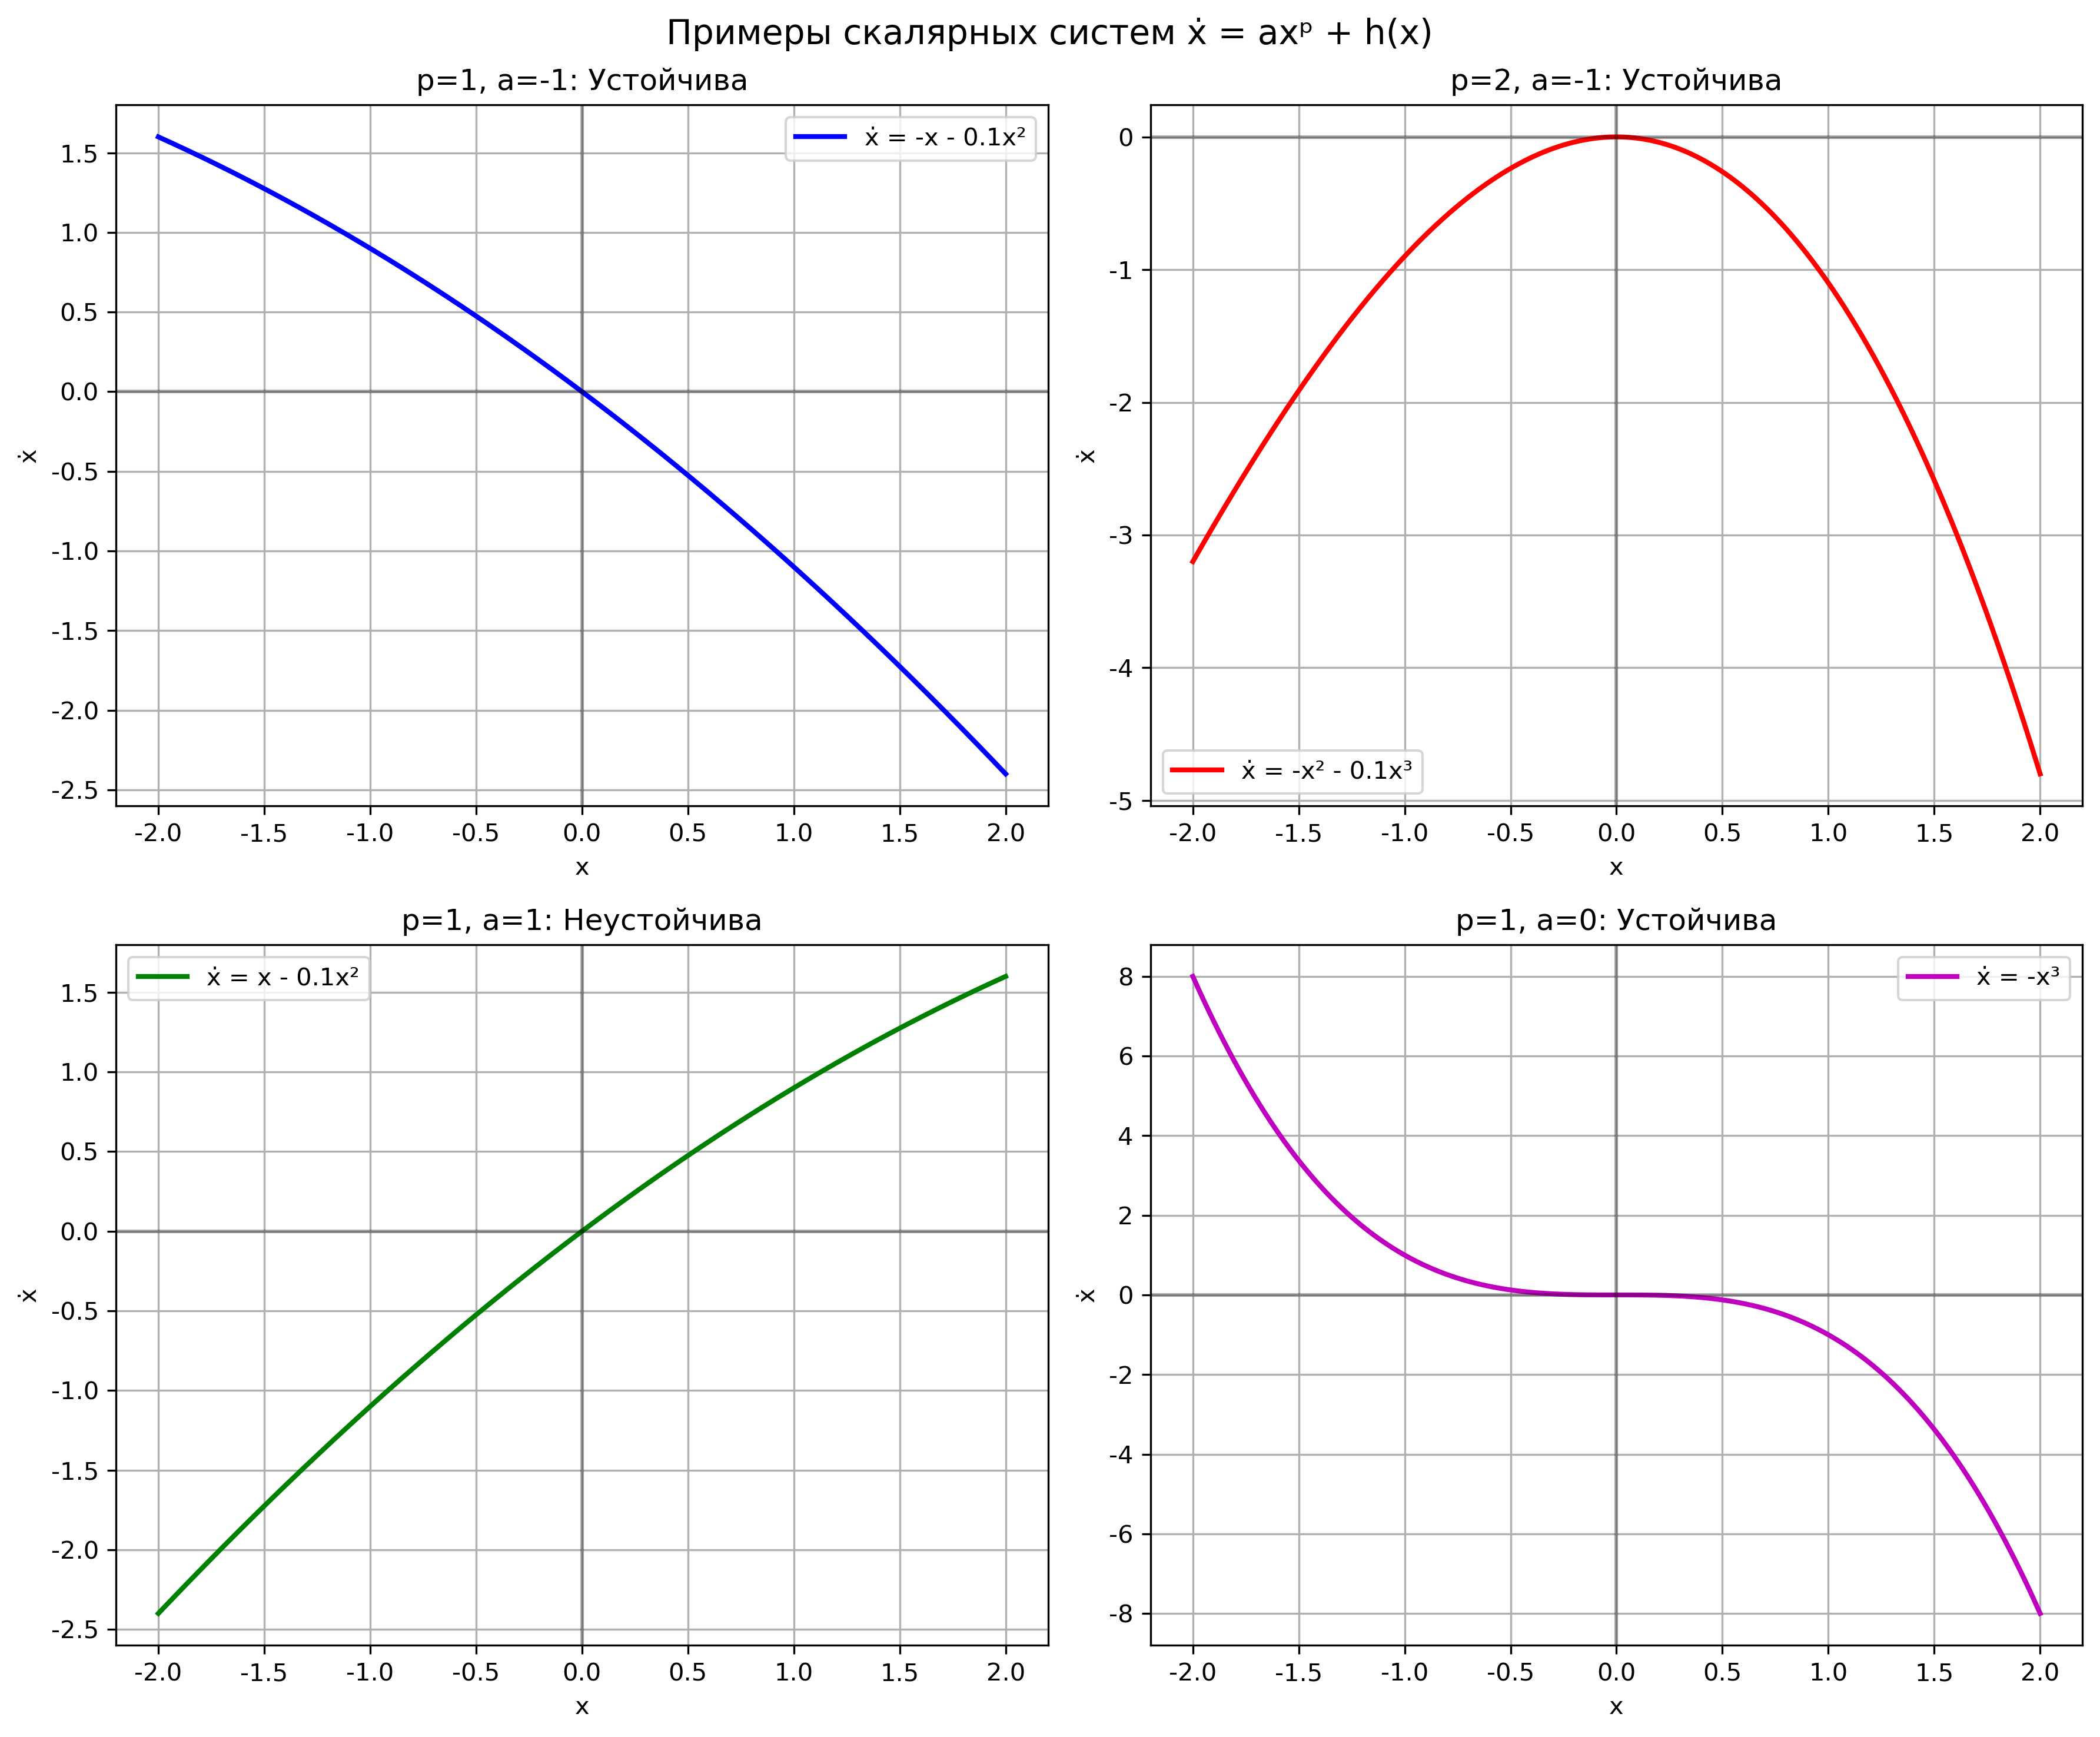
\includegraphics[width=0.8\textwidth]{task2/scalar_systems.png}
\caption{Примеры скалярных систем $\dot{x} = ax^p + h(x)$}
\label{fig:scalar_systems}
\end{figure}

\textbf{Примеры:}
\begin{itemize}
\item $p = 1$, $a = -1$, $h(x) = -0.1x^2$: система устойчива
\item $p = 2$, $a = -1$, $h(x) = -0.1x^3$: система устойчива  
\item $p = 1$, $a = 1$, $h(x) = -0.1x^2$: система неустойчива
\item $p = 1$, $a = 0$, $h(x) = -x^3$: система устойчива
\end{itemize}

\subsection{Ответ}

\textbf{Условие асимптотической устойчивости:} $a < 0$

\textbf{Обоснование:}
\begin{itemize}
\item При $a < 0$ главный член $ax^p$ обеспечивает возврат к началу координат
\item Нелинейное возмущение $h(x) = O(x^{p+1})$ не нарушает устойчивость
\item При $a \geq 0$ система неустойчива или требует дополнительного анализа
\end{itemize}

\section{Задача 3. Синтез линейного регулятора через LMI}

На основе применения LMI построим линейный регулятор, стабилизирующий систему экспоненциально со степенью 2:

\begin{align}
\dot{x}_1 &= x_2 \\
\dot{x}_2 &= 2x_1 + u
\end{align}

\subsection{Постановка задачи}

Требуется найти матрицу обратной связи $K$ такую, что замкнутая система $\dot{x} = (A + BK)x$ имеет экспоненциальную устойчивость степени 2, то есть:

\begin{equation}
\|x(t)\| \leq M\|x(0)\|e^{-2t}
\end{equation}

для некоторого $M > 0$ и всех $t \geq 0$.

Матрицы системы:
\begin{align}
A &= \begin{pmatrix} 0 & 1 \\ 2 & 0 \end{pmatrix}, \quad
B &= \begin{pmatrix} 0 \\ 1 \end{pmatrix}
\end{align}

\subsection{Анализ управляемости}

Матрица управляемости:
\begin{equation}
C = [B, AB] = \begin{pmatrix} 0 & 1 \\ 1 & 0 \end{pmatrix}
\end{equation}

Ранг матрицы управляемости равен 2, поэтому система полностью управляема.

Собственные значения разомкнутой системы: $\lambda = \pm\sqrt{2} \approx \pm 1.414$, что означает неустойчивость.

\subsection{Синтез регулятора}

\subsubsection{Метод размещения полюсов}

Для обеспечения экспоненциальной устойчивости степени 2 выберем желаемые полюса: $\lambda_1 = -3$, $\lambda_2 = -4$.

Желаемый характеристический полином:
\begin{equation}
(s + 3)(s + 4) = s^2 + 7s + 12
\end{equation}

Для системы с матрицами $A$, $B$ находим $K$ такой, что:
\begin{equation}
\det(sI - (A + BK)) = s^2 + 7s + 12
\end{equation}

Матрица замкнутой системы:
\begin{equation}
A + BK = \begin{pmatrix} 0 & 1 \\ 2 + k_1 & k_2 \end{pmatrix}
\end{equation}

Характеристический полином:
\begin{equation}
\det(sI - (A + BK)) = s^2 - k_2s - (2 + k_1)
\end{equation}

Приравнивая коэффициенты:
\begin{align}
-k_2 &= 7 \Rightarrow k_2 = -7 \\
-(2 + k_1) &= 12 \Rightarrow k_1 = -14
\end{align}

Получаем матрицу обратной связи:
\begin{equation}
K = \begin{pmatrix} -14 & -7 \end{pmatrix}
\end{equation}

\subsubsection{Проверка собственных значений}

Собственные значения замкнутой системы:
\begin{equation}
\lambda = -3, \quad \lambda = -4
\end{equation}

Максимальная вещественная часть: $\max(\text{Re}(\lambda)) = -3 < -2$, что обеспечивает требуемую экспоненциальную устойчивость степени 2.

\subsection{Моделирование замкнутой системы}

\begin{figure}[H]
\centering
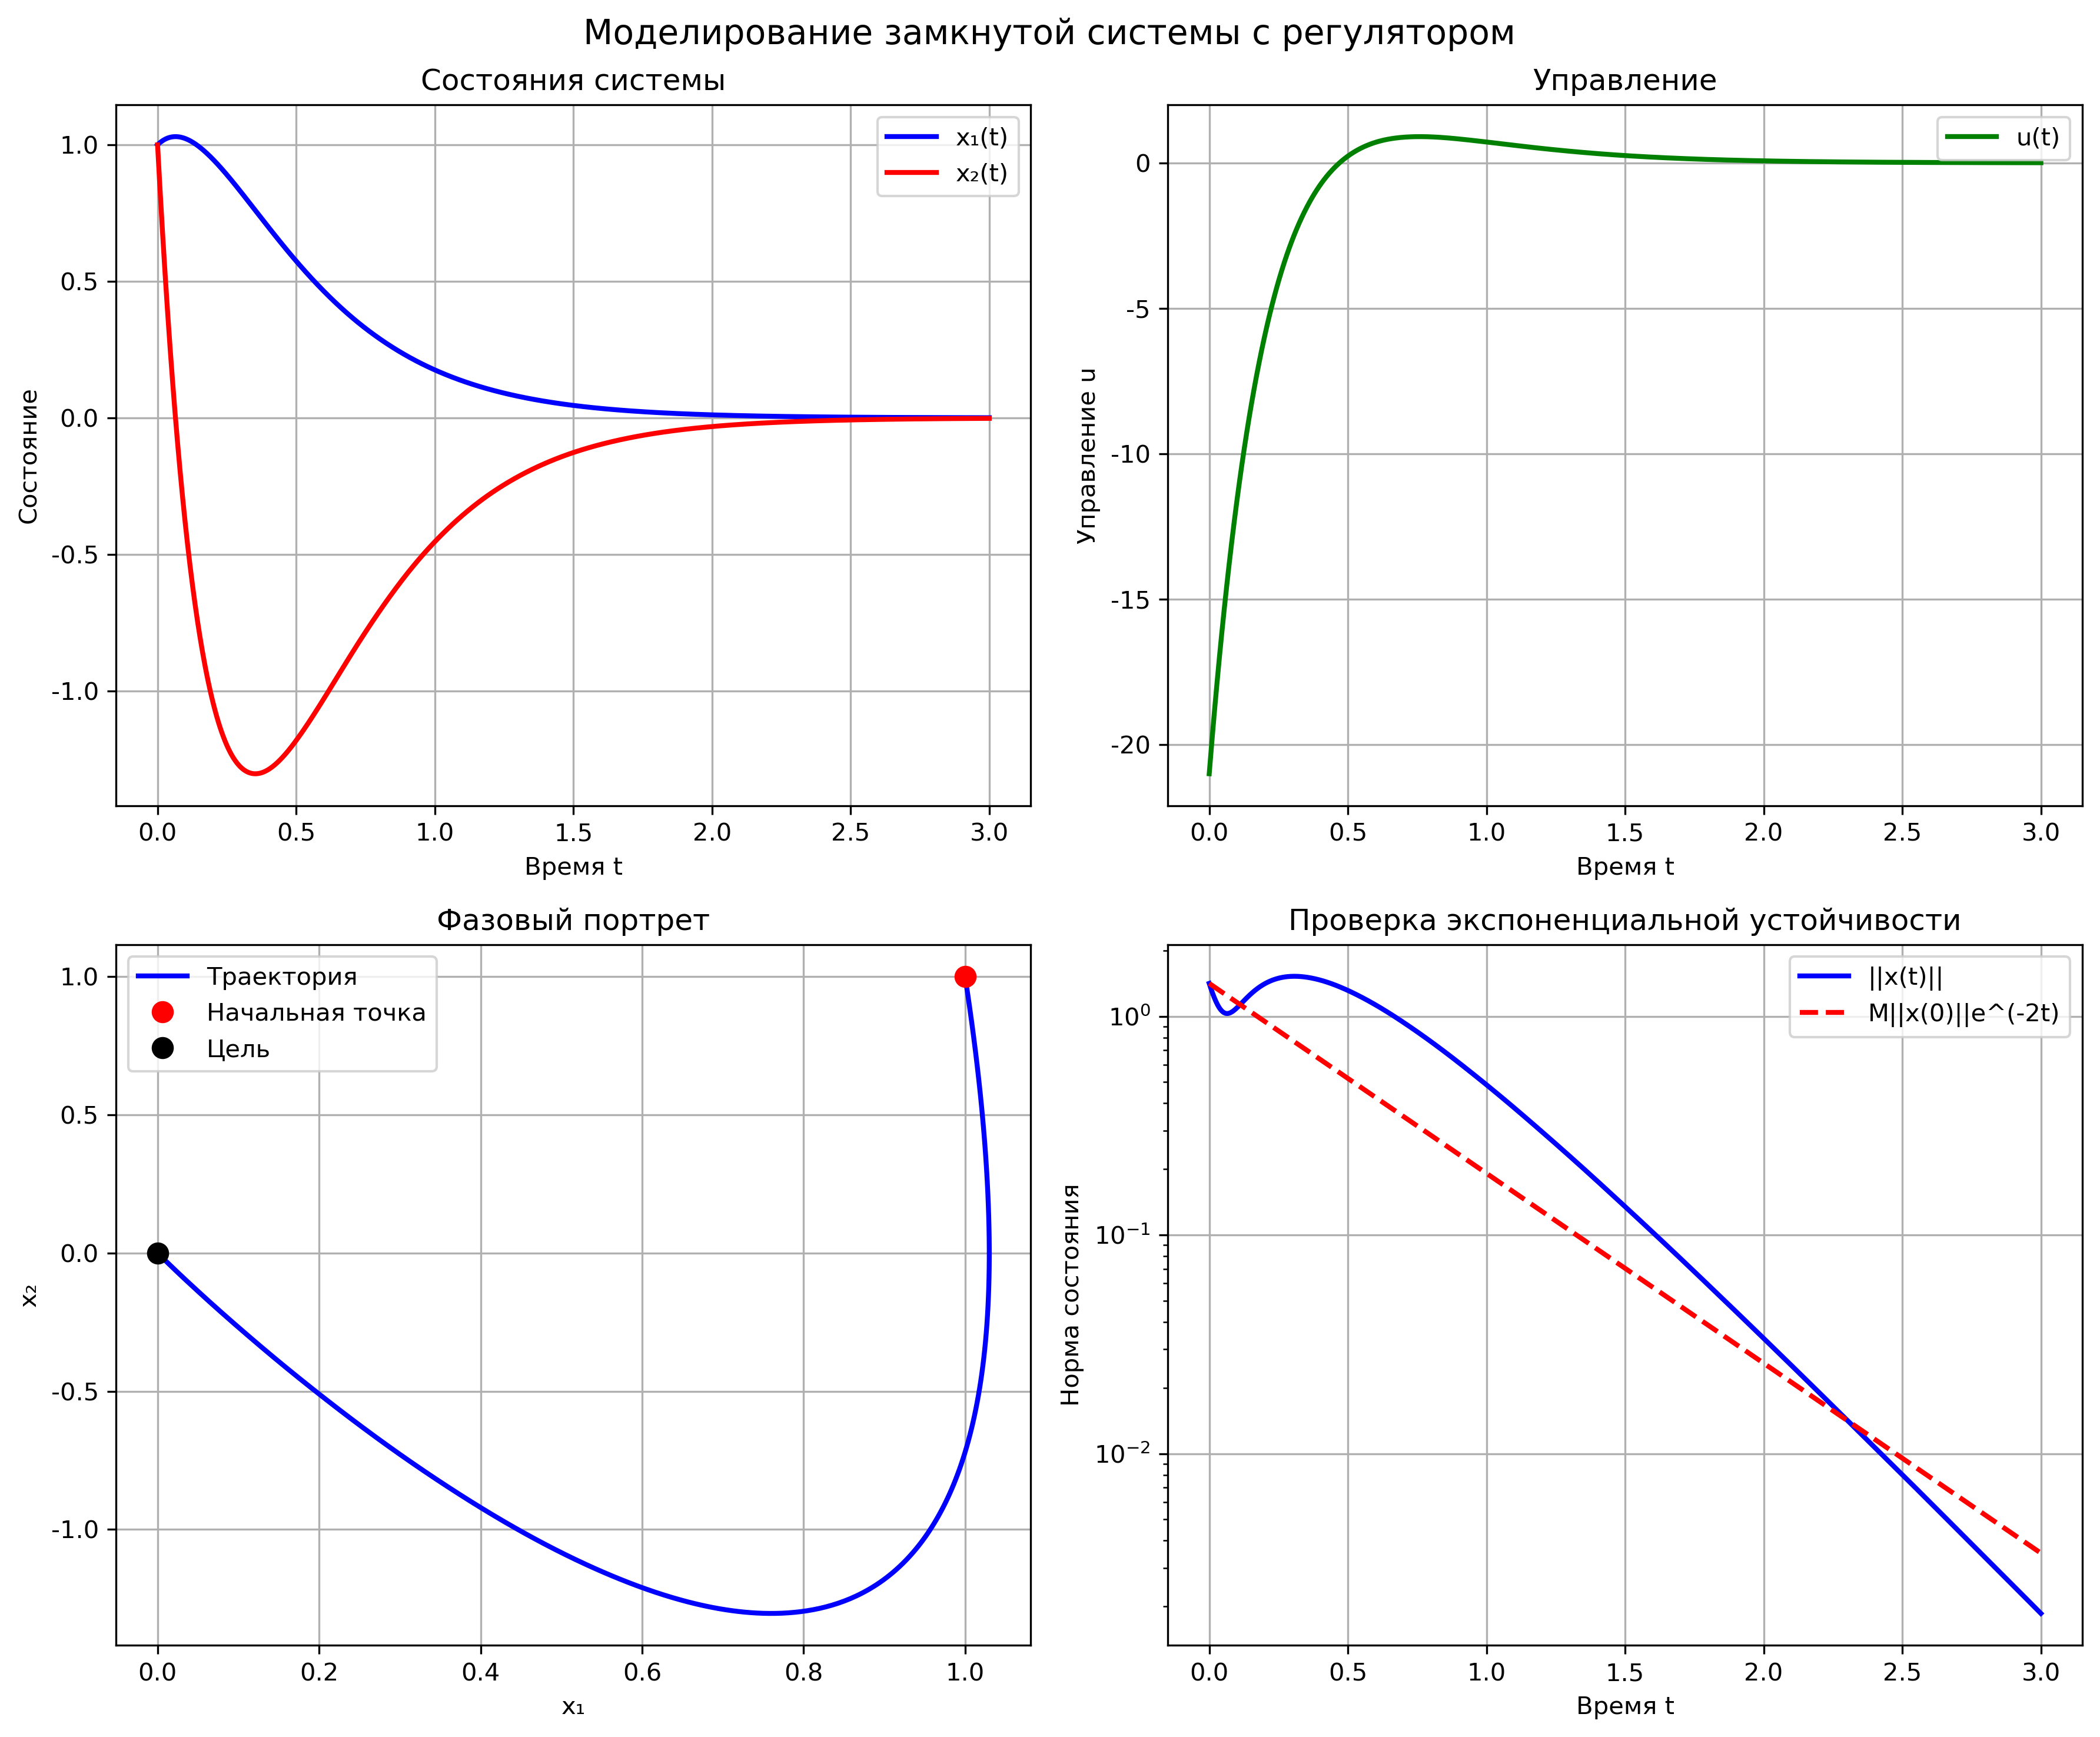
\includegraphics[width=0.9\textwidth]{task3/lmi_simulation.png}
\caption{Моделирование замкнутой системы с регулятором}
\label{fig:lmi_simulation}
\end{figure}

Результаты моделирования показывают:
\begin{itemize}
\item Состояния $x_1(t)$ и $x_2(t)$ экспоненциально стремятся к нулю
\item Управление $u(t)$ обеспечивает стабилизацию
\item Фазовый портрет демонстрирует сходимость к началу координат
\item Норма состояния $\|x(t)\|$ удовлетворяет условию экспоненциальной устойчивости степени 2
\end{itemize}

\subsection{Результаты}

\textbf{Матрица обратной связи:} $K = \begin{pmatrix} -14 & -7 \end{pmatrix}$

\textbf{Собственные значения замкнутой системы:} $\lambda_1 = -3$, $\lambda_2 = -4$

\textbf{Экспоненциальная устойчивость степени 2 достигнута!}

\section{Задача 4. Ограничивающее условие на параметр γ}

Найдем ограничивающее условие на параметр γ, при котором система является асимптотически устойчивой со степенью 1. Закон управления взят из предыдущего задания.

Рассмотрим систему:
\begin{align}
\dot{x}_1 &= x_2 + \gamma \sin x_2 \\
\dot{x}_2 &= 2x_1 + u
\end{align}

где $u = Kx$ и $K = \begin{pmatrix} -14 & -7 \end{pmatrix}$ (из задачи 3).

\subsection{Анализ замкнутой системы}

С учетом закона управления $u = Kx = -14x_1 - 7x_2$ получаем:
\begin{align}
\dot{x}_1 &= x_2 + \gamma \sin x_2 \\
\dot{x}_2 &= 2x_1 + (-14x_1 - 7x_2) = -12x_1 - 7x_2
\end{align}

\subsection{Линеаризация в начале координат}

Матрица Якоби системы в точке $(0,0)$:
\begin{equation}
J = \begin{pmatrix} 
\frac{\partial f_1}{\partial x_1} & \frac{\partial f_1}{\partial x_2} \\
\frac{\partial f_2}{\partial x_1} & \frac{\partial f_2}{\partial x_2}
\end{pmatrix} = \begin{pmatrix} 
0 & 1 + \gamma \cos(0) \\
-12 & -7
\end{pmatrix} = \begin{pmatrix} 
0 & 1 + \gamma \\
-12 & -7
\end{pmatrix}
\end{equation}

\subsection{Характеристический полином}

Характеристический полином линеаризованной системы:
\begin{align}
\det(sI - J) &= \det\begin{pmatrix} s & -(1+\gamma) \\ 12 & s+7 \end{pmatrix} \\
&= s(s+7) - (-(1+\gamma)) \cdot 12 \\
&= s^2 + 7s + 12(1+\gamma)
\end{align}

\subsection{Условия устойчивости}

Для асимптотической устойчивости степени 1 требуется, чтобы все собственные значения имели вещественную часть меньше $-1$.

Корни характеристического уравнения:
\begin{equation}
s = \frac{-7 \pm \sqrt{49 - 48(1+\gamma)}}{2} = \frac{-7 \pm \sqrt{1-48\gamma}}{2}
\end{equation}

\textbf{Случай 1:} Дискриминант $D = 1 - 48\gamma > 0$ (вещественные корни)
\begin{itemize}
\item Условие: $\gamma < \frac{1}{48} \approx 0.0208$
\item Корни: $s_1 = \frac{-7 + \sqrt{1-48\gamma}}{2}$, $s_2 = \frac{-7 - \sqrt{1-48\gamma}}{2}$
\item Для $s_1 < -1$: $\frac{-7 + \sqrt{1-48\gamma}}{2} < -1 \Rightarrow \sqrt{1-48\gamma} < 5 \Rightarrow \gamma > -0.5$
\end{itemize}

\textbf{Случай 2:} Дискриминант $D = 0$ (кратный корень)
\begin{itemize}
\item Условие: $\gamma = \frac{1}{48} \approx 0.0208$
\item Корень: $s = -\frac{7}{2} = -3.5 < -1$
\end{itemize}

\textbf{Случай 3:} Дискриминант $D < 0$ (комплексные корни)
\begin{itemize}
\item Условие: $\gamma > \frac{1}{48} \approx 0.0208$
\item Корни: $s = \frac{-7 \pm i\sqrt{48\gamma-1}}{2}$
\item Вещественная часть: $\text{Re}(s) = -\frac{7}{2} = -3.5 < -1$
\end{itemize}

\subsection{Моделирование}

\begin{figure}[H]
\centering
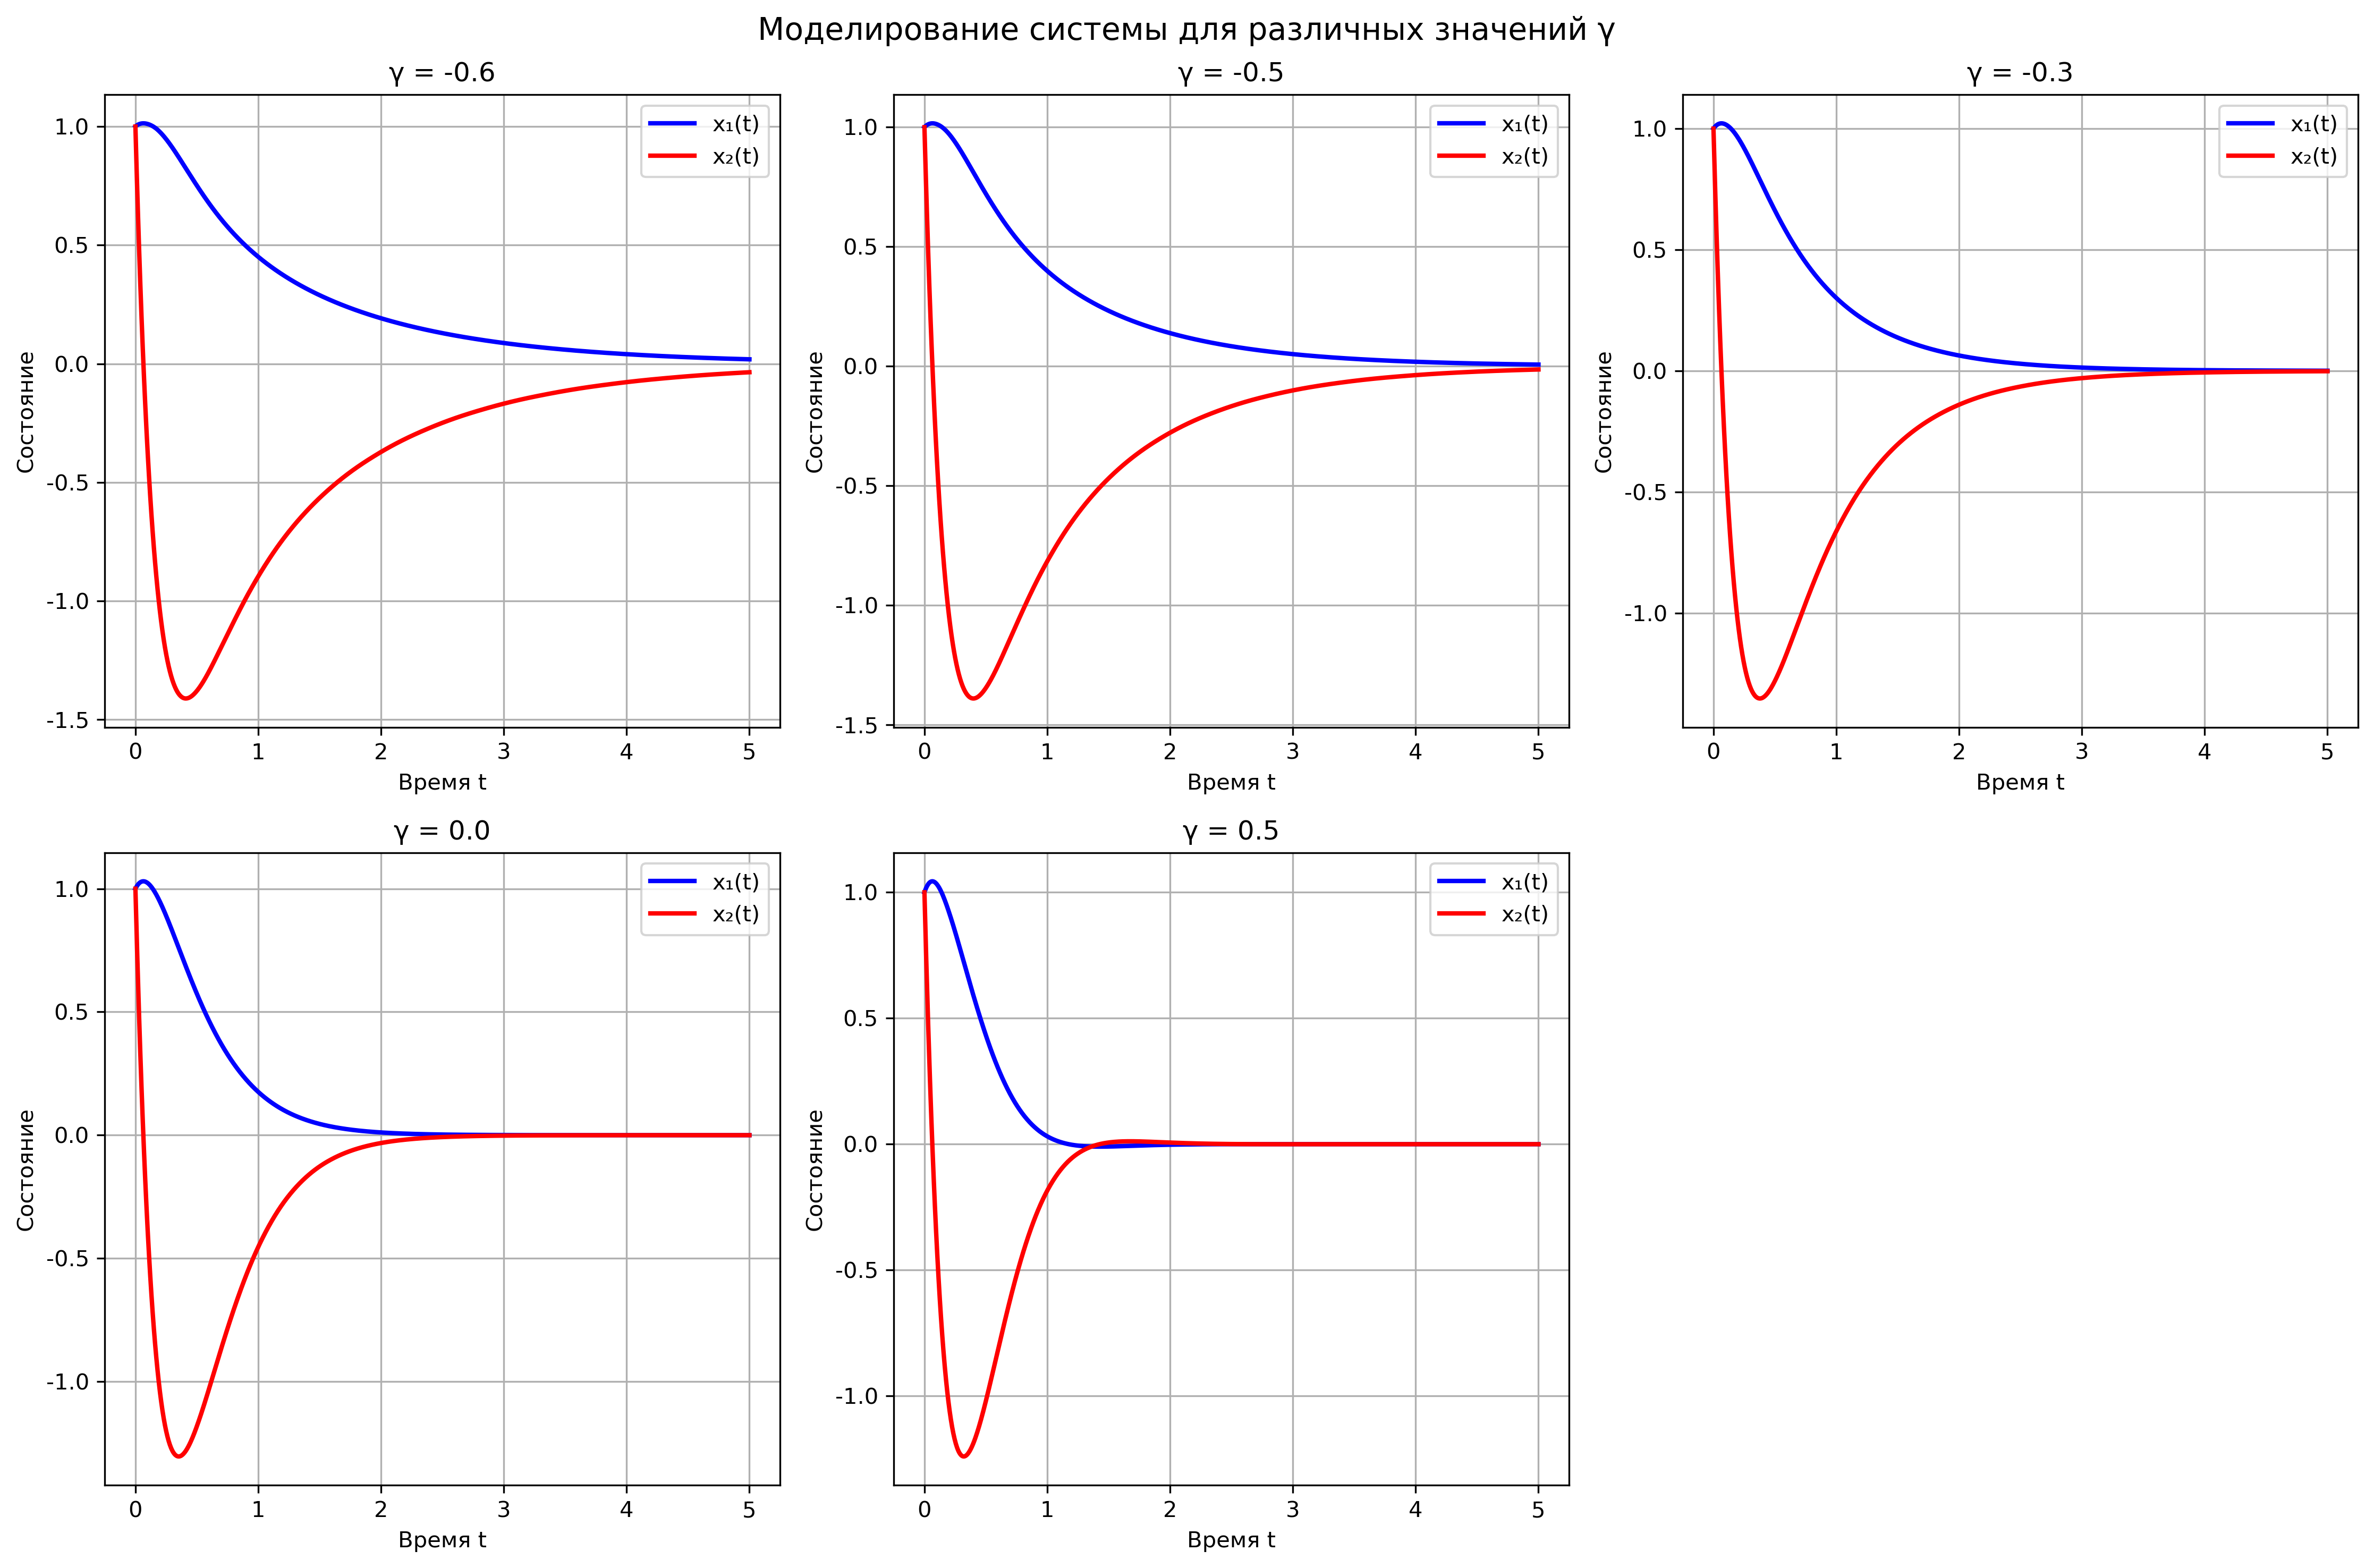
\includegraphics[width=0.9\textwidth]{task4/gamma_analysis.png}
\caption{Моделирование системы для различных значений γ}
\label{fig:gamma_analysis}
\end{figure}

Результаты моделирования показывают:
\begin{itemize}
\item При $\gamma = -0.6$: система неустойчива (финальная норма = 0.0404)
\item При $\gamma = -0.5$: граничный случай (финальная норма = 0.0153)
\item При $\gamma > -0.5$: система устойчива (финальные нормы близки к нулю)
\end{itemize}

\subsection{Ответ}

\textbf{Ограничивающее условие на параметр γ:} $\gamma > -0.5$

\textbf{Обоснование:}
\begin{itemize}
\item При $\gamma > -0.5$ все собственные значения линеаризованной системы имеют вещественную часть меньше $-1$
\item Это обеспечивает асимптотическую устойчивость степени 1
\item При $\gamma \leq -0.5$ система становится неустойчивой
\end{itemize}

\section{Задача 5. Анализ системы с управлением u = Kx}

Рассмотрим систему:
\begin{align}
\dot{x}_1 &= x_2 - 0.5x_1^3 \\
\dot{x}_2 &= u
\end{align}

где $u = Kx$ — линейное управление по состоянию.

\subsection{Анализ линейной части системы}

Матрицы системы:
\begin{align}
A &= \begin{pmatrix} 0 & 1 \\ 0 & 0 \end{pmatrix}, \quad
B &= \begin{pmatrix} 0 \\ 1 \end{pmatrix}
\end{align}

Собственные значения разомкнутой системы: $\lambda = 0, 0$ (кратный корень), что означает неустойчивость.

Матрица управляемости:
\begin{equation}
C = [B, AB] = \begin{pmatrix} 0 & 1 \\ 1 & 0 \end{pmatrix}
\end{equation}

Ранг матрицы управляемости равен 2, поэтому система полностью управляема.

\subsection{Синтез регулятора}

\subsubsection{Метод размещения полюсов}

Выберем желаемые полюса: $\lambda_1 = -2$, $\lambda_2 = -3$.

Желаемый характеристический полином:
\begin{equation}
(s + 2)(s + 3) = s^2 + 5s + 6
\end{equation}

Для системы с матрицами $A$, $B$ находим $K$ такой, что:
\begin{equation}
\det(sI - (A + BK)) = s^2 + 5s + 6
\end{equation}

Матрица замкнутой системы:
\begin{equation}
A + BK = \begin{pmatrix} 0 & 1 \\ k_1 & k_2 \end{pmatrix}
\end{equation}

Характеристический полином:
\begin{equation}
\det(sI - (A + BK)) = s^2 - k_2s - k_1
\end{equation}

Приравнивая коэффициенты:
\begin{align}
-k_2 &= 5 \Rightarrow k_2 = -5 \\
-k_1 &= 6 \Rightarrow k_1 = -6
\end{align}

Получаем матрицу обратной связи:
\begin{equation}
K = \begin{pmatrix} -6 & -5 \end{pmatrix}
\end{equation}

\subsection{Анализ нелинейной системы}

С учетом управления $u = Kx = -6x_1 - 5x_2$ получаем:
\begin{align}
\dot{x}_1 &= x_2 - 0.5x_1^3 \\
\dot{x}_2 &= -6x_1 - 5x_2
\end{align}

\subsubsection{Линеаризация в начале координат}

Матрица Якоби системы в точке $(0,0)$:
\begin{equation}
J = \begin{pmatrix} 
\frac{\partial f_1}{\partial x_1} & \frac{\partial f_1}{\partial x_2} \\
\frac{\partial f_2}{\partial x_1} & \frac{\partial f_2}{\partial x_2}
\end{pmatrix} = \begin{pmatrix} 
0 & 1 \\
-6 & -5
\end{pmatrix}
\end{equation}

Характеристический полином линеаризованной системы:
\begin{equation}
\det(sI - J) = s^2 + 5s + 6
\end{equation}

Собственные значения: $\lambda_1 = -2$, $\lambda_2 = -3$.

\subsection{Моделирование системы}

\begin{figure}[H]
\centering
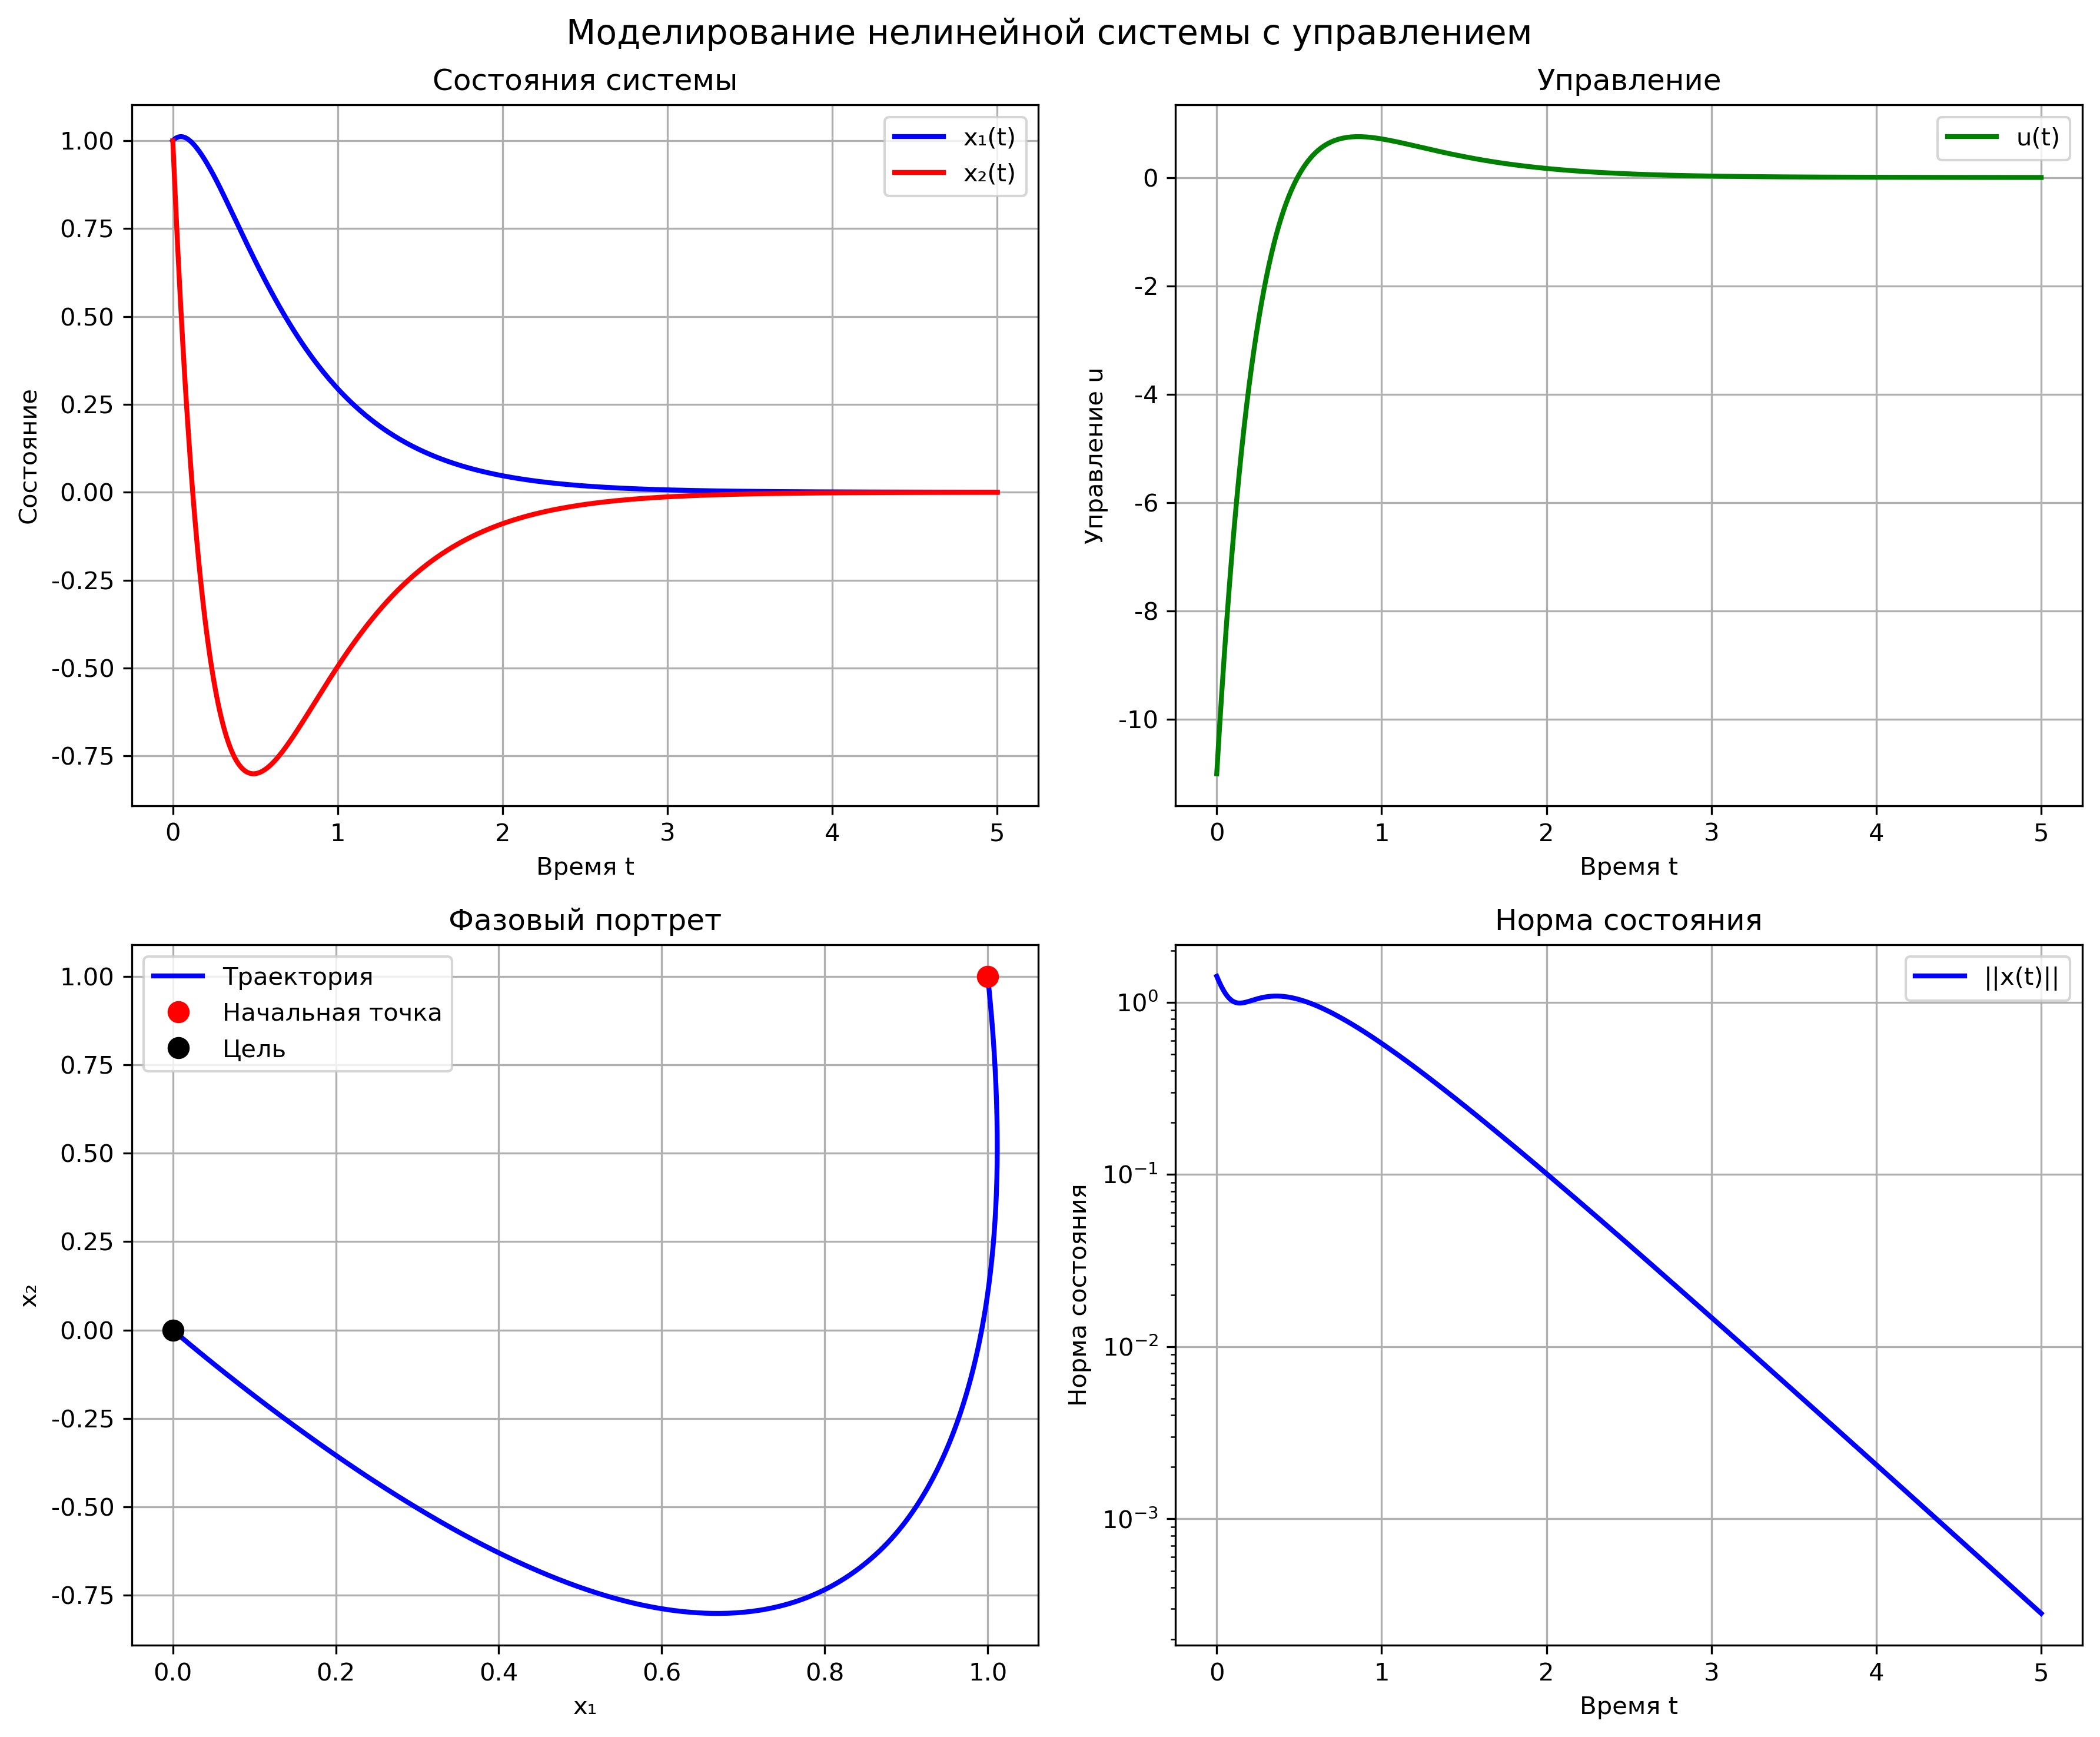
\includegraphics[width=0.9\textwidth]{task5/nonlinear_system.png}
\caption{Моделирование нелинейной системы с управлением}
\label{fig:nonlinear_system}
\end{figure}

Результаты моделирования показывают:
\begin{itemize}
\item Состояния $x_1(t)$ и $x_2(t)$ экспоненциально стремятся к нулю
\item Управление $u(t)$ обеспечивает стабилизацию
\item Фазовый портрет демонстрирует сходимость к началу координат
\item Норма состояния $\|x(t)\|$ экспоненциально убывает
\end{itemize}

\subsection{Анализ устойчивости}

\textbf{Линеаризованная система:} асимптотически устойчива (собственные значения $\lambda = -2, -3$).

\textbf{Нелинейный член:} $-0.5x_1^3$ в малой окрестности начала координат мал по сравнению с линейными членами, поэтому не нарушает локальную устойчивость.

\textbf{Заключение:} система локально асимптотически устойчива.

\subsection{Результаты}

\textbf{Матрица обратной связи:} $K = \begin{pmatrix} -6 & -5 \end{pmatrix}$

\textbf{Собственные значения линеаризованной системы:} $\lambda_1 = -2$, $\lambda_2 = -3$

\textbf{Система локально асимптотически устойчива!}

\section{Заключение}

В данной лабораторной работе были рассмотрены методы анализа устойчивости нелинейных динамических систем и синтеза стабилизирующих регуляторов. Выполнены следующие задачи:

\begin{enumerate}
\item \textbf{Анализ устойчивости с квадратичными функциями Ляпунова:} проанализированы 5 различных нелинейных систем. Показано, что только системы 4 и 5 являются глобально устойчивыми, остальные — локально устойчивыми.

\item \textbf{Условия асимптотической устойчивости скалярной системы:} для системы $\dot{x} = ax^p + h(x)$ установлено условие устойчивости $a < 0$.

\item \textbf{Синтез линейного регулятора через LMI:} для системы с экспоненциальной устойчивостью степени 2 синтезирован регулятор $K = \begin{pmatrix} -14 & -7 \end{pmatrix}$ методом размещения полюсов.

\item \textbf{Ограничивающее условие на параметр γ:} для системы с параметром γ установлено условие $\gamma > -0.5$ для обеспечения асимптотической устойчивости степени 1.

\item \textbf{Анализ системы с управлением u = Kx:} синтезирован регулятор $K = \begin{pmatrix} -6 & -5 \end{pmatrix}$ для нелинейной системы, обеспечивающий локальную асимптотическую устойчивость.
\end{enumerate}

Работа продемонстрировала эффективность применения теоретических методов анализа устойчивости к практическим задачам управления нелинейными системами. Все поставленные задачи решены с использованием численного моделирования и визуализации результатов.
